\section{Introducción}
\subsection*{Realidad aumentada}
\begin{frame}{Realidad aumentada}
\small{Un sistema de realidad aumentada (RA) reemplaza parte del mundo real con objetos virtuales, los cuales parecen coexistir en el mismo espacio que el ambiente real.}
\note[item]{$\rightarrow$ se crea una realidad mixta en tiempo real.}
  \begin{itemize}
    \item<1-> Introduce elementos virtuales en una escena captada de un entorno real.
    \item<2-> Trabaja interactivamente y en tiempo real.
    \item<3-> Detecta y realiza un ``seguimiento'' de objetos reales y virtuales entre sí.
    \item<4-> Realidad Aumentada no es Realidad Virtual.
    \item<5-> Según el grado de realismo o artificialidad:
    \begin{figure}[tbhp]
      \begin{centering}
	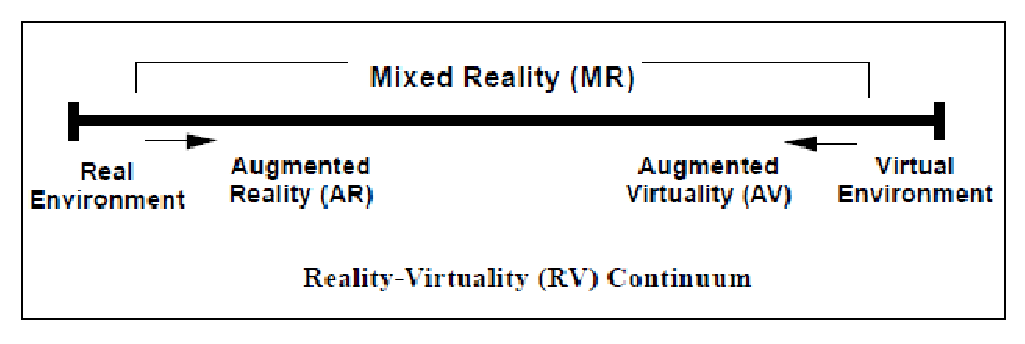
\includegraphics[width=6cm]{../../../img_ent1/reality_virtual.eps}
	\caption*{\tiny{Diagrama continuo de Realidad-Virtualidad. Milgram et al.}}
      \end{centering}
    \end{figure}
  \end{itemize}
\end{frame}

\begin{frame}{Sistemas y métodos para detección en RA}
    \begin{block}{Tipos de sistemas}
      \begin{itemize}
	    \item Basada en marcadores. \note[item]{es una imagen sintetica que altera el ambiente}
	    \item \textbf{No basada en marcadores} $\rightarrow$ características naturales de los objetos.
	      \note[item]{Marcelo: las características son de los objetos y NO DE LAS IMÁGENES}
      \end{itemize}
    \end{block}
   
     \begin{block}{Métodos para detección y seguimiento de objetos}
	\begin{itemize}
		\item Seguimiento basado en localización (GPS, acelerómetros, giroscopios, etc.)
		\item \textbf{Seguimiento óptico} $\rightarrow$ análisis e identificación de características a partir de la imagen.
		\item Una combinación de los dos anteriores.
	\end{itemize}
     \end{block}
\end{frame}

\begin{frame}{Aplicaciones - Ejemplos}
    \note[item]{Decir "marcadores" y  no patrónes!}
	\begin{center}{Aplicaciones - Ejemplos}
	  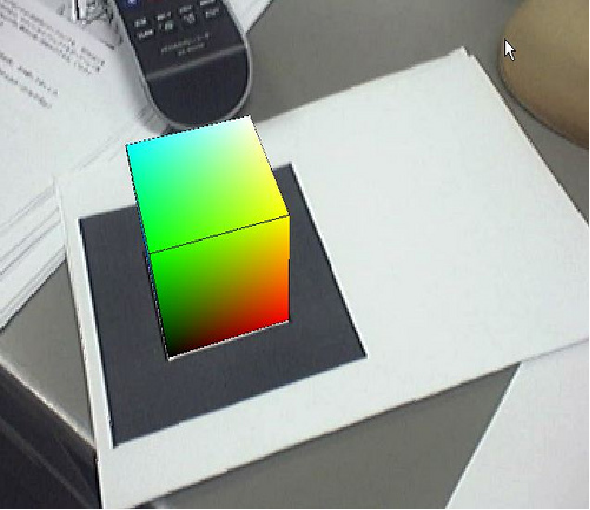
\includegraphics[width=7cm]{./img1/objeto_y_patron}
  	  
\includegraphics[width=7cm]{./img1/patrones}
	\end{center}
\end{frame}

\begin{frame}{Aplicaciones - Ejemplos}
      \note[item]{Decir "marcadores" y  no patrónes!}
	\begin{center}
	  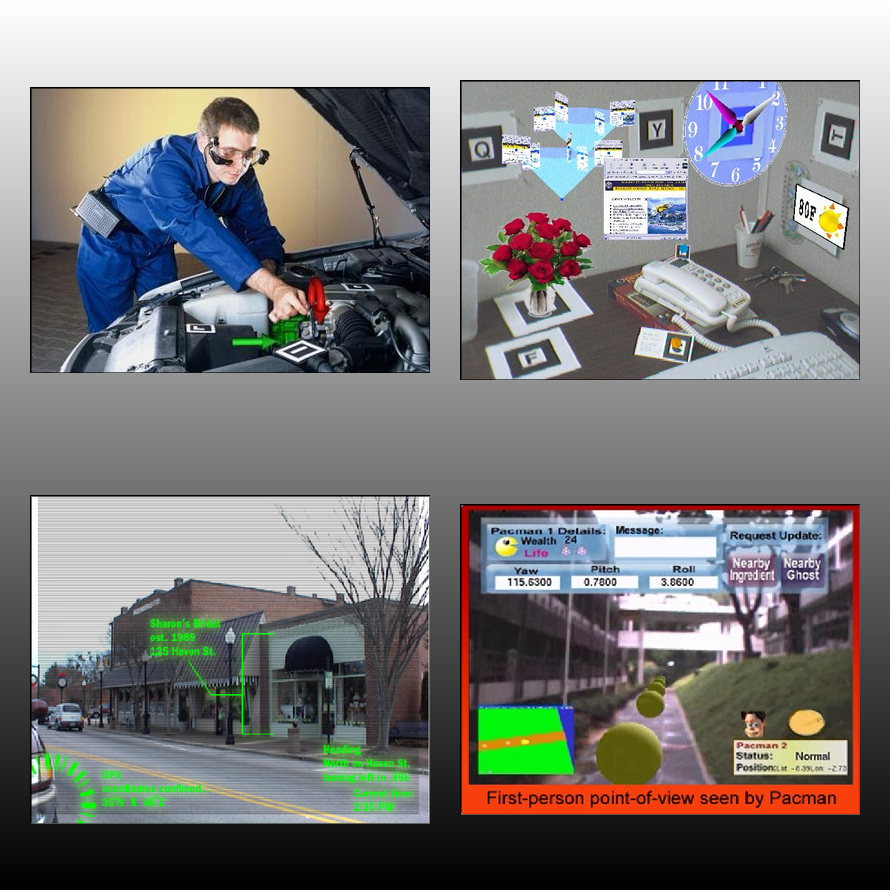
\includegraphics[width=7cm]{./img1/aplic1}
	\end{center}
\end{frame}
%%%%%%%%%%%%%%%%%%%%%%%%%%%%%%%%%%%%%%%%%%%%%%%%%%%%%%%%%
\subsection*{}
\begin{frame}{Motivación}
  \begin{itemize}
  \note[item]{Construir un método que permita reconocer objetos planos e identificar su posición en la imagen, en un ambiente controlado, para la posterior aplicación de realidad aumentada.}
  \item Desarrollo de un software propio de RA adaptable a aplicaciones específicas (comerciales, educativas, lúdicas, etc.)\footnote{SINC: Centro de Investigación en señales, sistemas e inteligencia computacional}
  \item No todas las aplicaciones trabajan en tiempo real.
  \item Muchos utilizan marcadores artificiales.
  \item Distribuidos bajo licencias privativas o costosos.
  \item Se trabaja con una tecnología que se encuentra en auge en estos tiempos.
      \note[item]{A cobrado gran imulso en el marketing, educación y e-commerce}
  \item El reconocimiento de objetos puede ser aplicado a diversidad de temáticas.
  \end{itemize}
\end{frame}

% \begin{frame}{Objetivos generales}
%   \begin{itemize}
%       \item Desarrollar un método para reconocer y seguir objetos en una secuencia de video digital y desarrollar un prototipo que haga uso del mismo aplicándolo a realidad aumentada.
%       \item Afianzar y extender los conocimientos adquiridos en el cursado de la carrera Ingeniería en Informática.
%   \end{itemize}
% \end{frame}
\subsection*{}
\begin{frame}
  \frametitle{Objetivos}
    \begin{itemize}
% 	\item Realizar el relevamiento del estado del arte en métodos utilizados para la detección y seguimiento de objetos en el Procesamiento Digital de imágenes.
	\item Diseñar y desarrollar un método reconocedor y seguidor de objetos planos en el flujo de video tomado por una cámara web estándar, sobre un ambiente controlado.
	\item Implementar el método en un algoritmo computacional que sea multiplataforma.
	%\item Optimizar el procesamiento llevado a cabo para lograr método desarrollado para que sea aplicable en tiempo real (\textbf{procesamiento}). 
	\item Optimizar el procesamiento para aplicarlo en tiempo real. 
	\item Implementar una aplicación prototipo específica (en el área de turismo, educación, publicidad, juegos u otros).
    \end{itemize}
\end{frame}

% \begin{frame}
% \frametitle{Alcances}
% \begin{itemize}
%   \item Se enmarcará en un sistema del tipo \textbf{sin marcadores} con método de reconocimiento del tipo \textbf{seguimiento óptico}.
%   \item El proyecto involucra el desarrollo de un prototipo para ser utilizado en una computadora con una cámara web estándar. Cabe aclarar, que no se pretende realizar una aplicación final específica y completa (estudio y diseño de interfaz amigable al usuario, introducción amigable de parámetros, etc.) orientada al uso de un usuario final.
%   \item Aunque no es un objetivo la implementación de varios métodos y su comparación, en una etapa previa se revisarán las características de algunos métodos para poder seleccionar alguno que se adecue a los requerimientos.
% \end{itemize}
% \end{frame}
%%